\documentclass[10pt,onecolumn]{article}

% ------------------------------------------------
% PAQUETES
% ------------------------------------------------
\usepackage[utf8]{inputenc}
\usepackage[T1]{fontenc}
\usepackage[spanish,es-tabla,es-nodecimaldot]{babel}
\usepackage{amsmath,amssymb}
\usepackage{graphicx}
\usepackage{geometry}
\usepackage{cite}
\usepackage{url}
\usepackage{titlesec}
\usepackage{abstract}
\usepackage{fancyhdr}

% ------------------------------------------------
% PAQUETES PARA ECUACIONES, FIGURAS Y GRÁFICAS
% ------------------------------------------------

\usepackage{mathtools}
\usepackage{bm}
\usepackage{siunitx}
\usepackage{float}
\usepackage{subcaption}
\usepackage{booktabs}
\usepackage{array}
\usepackage{multirow}
\usepackage{xcolor}

% Gráficas científicas
\usepackage{pgfplots}
\pgfplotsset{compat=1.18}

% Hipervínculos y referencias
\usepackage[colorlinks=true,
            linkcolor=blue,
            citecolor=blue,
            urlcolor=blue]{hyperref}

% Configuración de numeración de ecuaciones
\numberwithin{equation}{section}

% Configuración de numeración de figuras y tablas
\numberwithin{figure}{section}
\numberwithin{table}{section}

% Espaciado de figuras
\setlength{\textfloatsep}{10pt}
\setlength{\floatsep}{8pt}
\setlength{\intextsep}{8pt}

% Formato de captions
\usepackage[font=small,
            labelfont=bf,
            justification=centering]{caption}

\sisetup{output-decimal-marker={.}, group-digits=false}
\graphicspath{{figuras/}}

% Párrafo de declaración de uso de IA al final de cada apartado
\newcommand{\usoia}[1]{%
 \par\smallskip\noindent{\footnotesize\textbf{Uso de IA en este apartado.} #1}\par}

% ------------------------------------------------
% CONFIGURACIÓN DE PÁGINA
% ------------------------------------------------
\geometry{
    letterpaper,
    left=1.7cm,
    right=1.7cm,
    top=2cm,
    bottom=2cm,
    columnsep=0.7cm
}

\setlength{\parindent}{1em}
\setlength{\emergencystretch}{1.5em}
\setlength{\parskip}{3pt}

\titleformat{\section}
{\normalfont\bfseries\normalsize}
{\thesection.}{0.5em}{}

\titleformat{\subsection}
{\normalfont\bfseries\small}
{\thesubsection}{0.5em}{}

% ------------------------------------------------
% INFORMACIÓN DEL PROYECTO
% ------------------------------------------------

\title{
    \textbf{\Large SEMP: DISEÑO Y SIMULACIÓN DE UN SENSOR ELECTROMAGNÉTICO DE PROXIMIDAD PARA LA DETECCIÓN,
    IDENTIFICACIÓN Y UBICACIÓN DE PIEZAS METÁLICAS}
}

\author{
    Luis Ernesto Rodríguez$^{1}$,
    Sebastián Santander Soto$^{1}$,
    Kevin Lozano Gómez$^{1}$,\\
    Juan Pablo Corchuelo$^{1}$,
    Mateo López$^{1}$\\[0.3cm]
    \small
    $^{1}$ Curso de Electromagnetismo,
    Universidad Icesi, Cali, Colombia\\
    \small
    Repositorio: \url{https://github.com/luisrodriguez-rgb/Proyecto-Final-Fisica}
}

\date{}

% ------------------------------------------------
% DOCUMENTO
% ------------------------------------------------

\begin{document}

% ------------------------------------------------
% TÍTULO Y AUTORES
% ------------------------------------------------

\twocolumn[
\begin{@twocolumnfalse}

\maketitle

% ------------------------------------------------
% RESUMEN
% ------------------------------------------------

\begin{center}
    \textbf{RESUMEN}
\end{center}

\noindent
Los sensores inductivos de proximidad detectan piezas metálicas sin contacto y son esenciales en la
automatización industrial. En este proyecto se modela, se resuelve y se simula un sensor de este tipo aplicado a
una línea de autopartes por la que pasan piezas de acero, cobre, aluminio, latón y acero inoxidable. Siguiendo el
esquema de Detección, Emisiones, Propiedades y Alerta (D.E.P.A.), el modelo parte de las leyes de Faraday y de
Ampère en régimen cuasi-estático: el campo variable de la bobina induce corrientes de Foucault en la pieza, que
modifican la inductancia y la resistencia efectivas de la bobina. Esos cambios se calculan con la solución
semianalítica de Dodd y Deeds y se introducen en un circuito RL, resuelto por la ley de mallas de Kirchhoff con el
mismo procedimiento que el circuito RC visto en clase. La ecuación diferencial se integra con los métodos de Euler
y Runge--Kutta de cuarto orden programados manualmente, cuyos órdenes de convergencia medidos (1.01 y 4.02)
coinciden con los teóricos. Se construyó un simulador interactivo en Python con Streamlit que permite variar el
número de espiras, la frecuencia, la distancia y el material. Los resultados muestran que el cobre reduce la
inductancia en un 8.5\,\% a 5~mm y que el acero la aumenta en un 5.5\,\%; que el alcance del sensor es del orden
del radio de la bobina; que el acero presenta una frecuencia ciega cerca de 20~kHz; y que la fase del cambio de
impedancia permite identificar el material con un 100\,\% de acierto cuando se mide con dos frecuencias y se
promedia la señal, estimando además la distancia con un error de 0.03~mm.

\vspace{0.2cm}
\noindent
\textbf{Palabras clave:} sensor inductivo, corrientes de Foucault, ley de Faraday, circuito RL, Runge--Kutta,
plano de impedancia.

\vspace{0.4cm}

\end{@twocolumnfalse}
]

% =================================================
% SECCIONES DEL PROYECTO
% =================================================

\section{Introducción}

En las líneas de producción es necesario detectar piezas metálicas sin tocarlas: contar tornillos, verificar la
posición de una carcasa o separar materiales. Los sensores inductivos de proximidad resuelven esta tarea con un
campo magnético variable y, a diferencia de los sensores ópticos o capacitivos, no les afectan el polvo, el aceite
ni la suciedad no metálica \cite{fericean2007,garcia2011}. Su principio es la inducción electromagnética: una
bobina alimentada con corriente alterna crea un campo que induce corrientes en la pieza, y la reacción de esas
corrientes cambia la impedancia de la bobina \cite{griffiths2017,libby1971}.

\textbf{Problema.} En una línea de autopartes pasan, mezclados, tornillos de acero, cables de cobre, carcasas de
aluminio, conectores de latón y abrazaderas de acero inoxidable. Un sensor que solo indique ``hay una pieza'' no
basta para clasificarlas. Se requiere además saber \emph{de qué metal es} cada pieza y \emph{a qué distancia}
pasa, y advertir cuando una pieza no corresponde a ningún material conocido.

\textbf{Propósito.} Modelar el sensor a partir de las ecuaciones de Maxwell, resolver el modelo analítica y
numéricamente, y construir un simulador que permita evaluar qué tan eficiente es la solución.

\textbf{Objetivos.}
\begin{enumerate}
 \item Deducir el modelo del sensor desde las leyes de Faraday y Ampère, y su circuito equivalente RL.
 \item Resolver analíticamente la respuesta del circuito a una fuente continua y a una fuente alterna.
 \item Implementar manualmente los métodos de Euler y Runge--Kutta de cuarto orden (RK4) y validar su
       convergencia frente a la solución exacta.
 \item Simular la detección, la identificación del material y la estimación de la distancia, y medir su
       exactitud.
\end{enumerate}

\textbf{Alcance.} El modelo trata la pieza como un semiespacio conductor, la bobina como un solenoide de capa
delgada sin núcleo y los materiales como lineales. El estudio se organiza con el esquema D.E.P.A. propuesto en
el curso: \emph{Detección} (qué detectar), \emph{Emisiones} (cómo responde la pieza), \emph{Propiedades} de los
campos (frecuencia, energía, potencia) y \emph{Alerta} (lo que entrega el sensor).

\usoia{Se usó Claude (Anthropic) para redactar un primer borrador de la introducción a partir de la guía y la
propuesta del curso. El equipo definió el problema, el caso de estudio y los objetivos, y revisó el texto.}

\section{Modelo teórico}

\subsection{Descripción del proceso}

El proceso se describe por etapas, como se hizo en clase con el espectrómetro de masas, para usar en cada una
solo la física que necesita:

\begin{enumerate}
 \item \textbf{Detección.} La bobina crea un campo magnético $\vec B(t)$ alrededor de su cara activa. Hay que
       decidir el material de la pieza y su distancia.
 \item \textbf{Emisiones.} El flujo variable induce en la pieza un campo eléctrico (ley de Faraday) que mueve
       las cargas libres: aparecen corrientes de Foucault $\vec J=\sigma\vec E$. Por la ley de Lenz, su campo se
       opone al de la bobina; parte del flujo deja de enlazarla y su inductancia disminuye. Las pérdidas por
       efecto Joule en la pieza aparecen como un aumento de la resistencia. Si la pieza es ferromagnética, además
       se magnetiza y concentra el flujo, lo que tiende a aumentar la inductancia.
 \item \textbf{Propiedades.} La respuesta depende de la frecuencia, que fija la profundidad de penetración, y de
       la potencia intercambiada con la pieza, que disminuye con la distancia.
 \item \textbf{Alerta.} El sistema compara la corriente medida con la esperada para cada material y entrega el
       material, la distancia o un aviso de impureza.
\end{enumerate}

\textbf{Variables.} Vectoriales: $\vec B$ (T), $\vec E$ (V/m), $\vec J$ (A/m$^2$) y el potencial vector
$\vec A$, con $\vec B=\nabla\times\vec A$. Escalares: la corriente $i(t)$ (A), la fem $\varepsilon(t)$ (V), la
inductancia $L$ (H), la resistencia $R$ ($\Omega$), el flujo $\Phi_B$ (Wb), la conductividad $\sigma$ (S/m), la
permeabilidad relativa $\mu_r$, la frecuencia angular $\omega$ y la geometría: espiras $N$, radio $a$, longitud
$l$ y distancia $d$.

\textbf{Hipótesis.} (i) Régimen cuasi-estático; (ii) materiales lineales, homogéneos e isótropos; (iii) bobina
de capa delgada sin capacitancia entre espiras; (iv) pieza más ancha que la bobina y más gruesa que $3\delta$;
(v) pieza que se mueve despacio frente al período de la fuente, de modo que para cada posición se usa una
inductancia constante.

\subsection{Fundamentación matemática}

\textbf{Ecuaciones de Maxwell necesarias.} Solo se emplean las que el sensor requiere \cite{griffiths2017,jackson1999}.
La ley de Faraday es la central:
\begin{equation}
 \oint_C \vec E\cdot d\vec l = -\frac{d\Phi_B}{dt},\qquad \Phi_B=\vec B\cdot\vec A .
 \label{eq:faraday}
\end{equation}
La ley de Ampère, sin corriente de desplazamiento, da los campos de la bobina y de la pieza:
\begin{equation}
 \oint_C \vec B\cdot d\vec l = \mu_0 I_{enc}.
 \label{eq:ampere}
\end{equation}
La corriente de desplazamiento se desprecia porque en el cobre a 1~kHz
$\omega\varepsilon_0/\sigma\approx9\times10^{-19}$, y porque la longitud de onda ($\lambda=c/f=300$~km) es
enorme frente a la bobina. La ley de Gauss para el magnetismo, $\oint\vec B\cdot d\vec A=0$, solo se usa como
condición de frontera. La ley de Gauss eléctrica no interviene: las corrientes de Foucault forman lazos cerrados
sin acumulación de carga. Combinando estas leyes con $\vec J=\sigma\vec E$, dentro del metal se obtiene una
ecuación de difusión,
\begin{equation}
 \nabla^2\vec A = j\omega\mu_0\mu_r\sigma\,\vec A ,
 \qquad
 \delta=\sqrt{\frac{2}{\omega\mu_0\mu_r\sigma}},
 \label{eq:difusion}
\end{equation}
donde $\delta$ es la profundidad de penetración: 2.06~mm para el cobre y 0.65~mm para el acero al carbono a 1~kHz.

\textbf{Inductancia de la bobina.} Aplicando la ley de Ampère a un solenoide ideal, $B=\mu_0Ni/l$; el flujo por
espira es $\Phi_B=B\pi a^2$, igual que el flujo eléctrico $\Phi=\vec E\cdot\vec A$ de la ley de Gauss. La
inductancia es la razón entre el flujo enlazado y la corriente, como la capacitancia es la razón entre carga y
potencial: $L=N\Phi_B/i=\mu_0N^2\pi a^2/l$. Para una bobina corta se usa la corrección de Wheeler \cite{wheeler1928}:
\begin{equation}
 L_0=\frac{\mu_0N^2\pi a^2}{l+0.9a}.
 \label{eq:wheeler}
\end{equation}

\textbf{Efecto de la pieza.} Dodd y Deeds resolvieron \eqref{eq:difusion} para una bobina sobre un semiespacio
conductor \cite{dodd1968}. El cambio de impedancia es
\begin{equation}
 \Delta Z=j\omega\pi\mu_0a^2N^2\!\int_0^\infty\! J_1^2(\alpha a)\,\Gamma(\alpha)\,F^2(\alpha)\,d\alpha,
 \label{eq:dodd}
\end{equation}
con $F(\alpha)=\left[e^{-\alpha d}-e^{-\alpha(d+l)}\right]/(\alpha l)$,
$\Gamma=(\mu_r\alpha-\alpha_1)/(\mu_r\alpha+\alpha_1)$ y $\alpha_1=\sqrt{\alpha^2+j\omega\mu_0\mu_r\sigma}$.
De ahí salen los parámetros efectivos:
\begin{equation}
 L_{\text{eff}}=L_0+\frac{\operatorname{Im}\Delta Z}{\omega},\qquad R_{\text{eff}}=R_0+\operatorname{Re}\Delta Z .
 \label{eq:efectivos}
\end{equation}
Para un conductor perfecto $\Gamma\to-1$ y la pieza actúa como un espejo que crea una bobina imagen con corriente
opuesta (método de las imágenes); para un ferromagnético no conductor $\Gamma=(\mu_r-1)/(\mu_r+1)>0$.

\textbf{Circuito RL.} Recorriendo la malla con la convención de signos de clase (fuente $+\varepsilon$, resistor
$-iR$, bobina $-L\,di/dt$ por la ley de Faraday), la ley de Kirchhoff da
\begin{equation}
 \varepsilon(t)-iR-L\frac{di}{dt}=0 .
 \label{eq:kirchhoff}
\end{equation}
Si la pieza se mueve, la inductancia depende del tiempo y \eqref{eq:kirchhoff} se generaliza aplicando Faraday
al flujo enlazado $L(t)\,i$:
\begin{equation}
\begin{aligned}
 \frac{di}{dt} &= \frac{\varepsilon(t)-\left[R(t)+\dot L(t)\right]i}{L(t)},\\
 \frac{dd}{dt} &= v(t).
\end{aligned}
\label{eq:sistema}
\end{equation}

\textbf{Solución analítica con fuente continua.} Con $\varepsilon=V_0$ e $i(0)=0$, \eqref{eq:kirchhoff} es separable,
como la carga del capacitor en el circuito RC \cite{serway2018}:
\begin{equation}
 \int_0^t\frac{dt}{\tau}=\int_0^{i}\frac{di}{i_{max}-i}
 \;\Rightarrow\;
 i(t)=i_{max}\left(1-e^{-t/\tau}\right),
 \label{eq:escalon}
\end{equation}
con $i_{max}=V_0/R$ y $\tau=L/R$. En $t=\tau$ se alcanza el 63\,\% de $i_{max}$. Al desenergizar
($\varepsilon=0$), $i(t)=i_s\,e^{-(t-t_s)/\tau}$. Multiplicando \eqref{eq:kirchhoff} por $i$ se obtiene el
balance de energía $\varepsilon i=i^2R+\frac{d}{dt}\left(\tfrac12Li^2\right)$.

\textbf{Solución analítica con fuente alterna.} Con $\varepsilon=V_0\sin\omega t$, por coeficientes
indeterminados (verificado con SymPy \cite{meurer2017}):
\begin{equation}
 i(t)=\left[I_0+I_p\sin\varphi\right]e^{-t/\tau}+I_p\sin(\omega t-\varphi),
 \label{eq:alterna}
\end{equation}
\begin{equation}
 I_p=\frac{V_0}{\sqrt{R^2+\omega^2L^2}},\qquad \varphi=\arctan\frac{\omega L}{R}.
 \label{eq:amplitud}
\end{equation}

\textbf{Detección e identificación.} Hay pieza cuando $|I_p-I_{p,0}|/I_{p,0}$ supera un umbral (2\,\%). Para
identificar el material se mide la amplitud y la fase de la corriente, se reconstruye
$Z=(V_0/I_p)e^{j\varphi}$ y se calcula $z=(Z-Z_0)/(\omega L_0)$. La fase de $z$ depende sobre todo del material y
de la frecuencia, y su magnitud de la distancia; es el método del plano de impedancia de los ensayos no
destructivos por corrientes de Foucault \cite{libby1971,garcia2011}.

\subsection{Representación del sistema}

La Figura \ref{fig:modelo} muestra la geometría del sensor y su circuito equivalente.

\begin{figure*}[t]
    \centering
    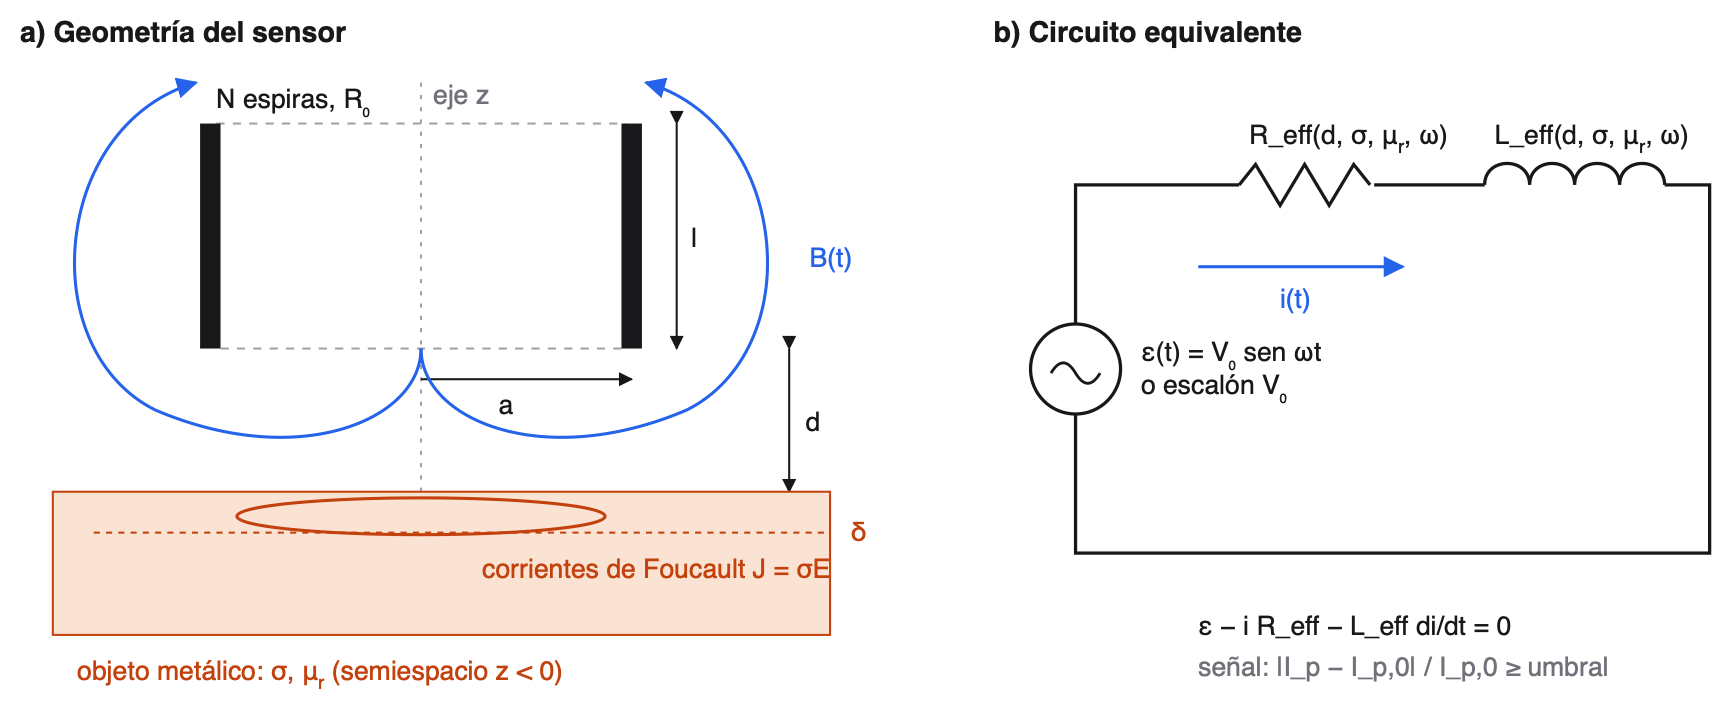
\includegraphics[width=0.78\textwidth]{modelo_teorico.png}
    \caption{a) Bobina de radio $a$ y longitud $l$ a una distancia $d$ de la pieza, con las corrientes de Foucault
    confinadas en una capa de espesor $\delta$. b) Circuito RL equivalente.}
    \label{fig:modelo}
\end{figure*}

\subsection{Condiciones iniciales y de frontera}

La condición inicial es la corriente de la bobina al conectarla:
\begin{equation}
 i(0)=I_0 ,
 \label{eq:condicion_inicial}
\end{equation}
con $I_0=0$ en los casos estudiados. Las condiciones de frontera en la superficie de la pieza ($z=0$) son la
continuidad de $B_z$ y de $H_\rho$, y los campos se anulan lejos de la bobina. En el caso de la pieza en
movimiento, $d(0)=d_{max}$.

\subsection{Caso de estudio}

La Tabla \ref{tab:caso} resume los materiales de la línea de autopartes. El sensor de referencia tiene $N=150$
espiras, $a=15$~mm, $l=20$~mm y $R_0=5~\Omega$, y se alimenta con $V_0=5$~V a 1~kHz (y a 5~kHz en la segunda
medición). Con \eqref{eq:wheeler}, $L_0=0.597$~mH y $\tau_0=L_0/R_0=119~\mu$s. Requisitos: avisar si una pieza
pasa a menos de 8~mm, identificar su material, estimar su distancia y avisar cuando no coincida con el catálogo.

\begin{table}[H]
    \centering
    \caption{Materiales del caso de estudio \cite{jackson1999}.}
    \label{tab:caso}
    \small
    \begin{tabular}{llcc}
        \toprule
        Pieza & Material & $\sigma$ (S/m) & $\mu_r$ \\
        \midrule
        Tornillos & Acero al carbono & $6.0\times10^{6}$ & 100 \\
        Cables & Cobre & $5.96\times10^{7}$ & 1 \\
        Carcasas & Aluminio & $3.77\times10^{7}$ & 1 \\
        Conectores & Latón & $1.5\times10^{7}$ & 1 \\
        Abrazaderas & Inoxidable 304 & $1.45\times10^{6}$ & 1.02 \\
        \bottomrule
    \end{tabular}
\end{table}

\usoia{Claude (Anthropic) se usó para buscar y explicar el modelo de Dodd y Deeds, redactar borradores de las
deducciones y comprobar el álgebra con SymPy. Las deducciones del circuito se contrastaron con los apuntes de
clase del circuito RC y la ley de Gauss; los valores numéricos se obtuvieron ejecutando el código del proyecto.}

\section{Implementación numérica}

Las ecuaciones \eqref{eq:kirchhoff} y \eqref{eq:sistema} son problemas de valor inicial de primer orden,
$i'=f(t,i)$, para los cuales los métodos de Euler y RK4 son adecuados \cite{burden2017,butcher2016}. La guía del
curso exige programarlos manualmente; \texttt{solve\_ivp} de SciPy \cite{virtanen2020} se usa solo como contraste.

\subsection{Método numérico empleado}

La derivada temporal se aproxima mediante diferencias finitas,
\begin{equation}
    \frac{di}{dt}
    \approx
    \frac{i_{n+1}-i_n}{\Delta t},
    \label{eq:diferencias_finitas}
\end{equation}
donde $\Delta t$ es el paso de tiempo. Para mayor precisión se usa además RK4, que promedia cuatro pendientes en
cada paso:
\begin{equation}
\begin{aligned}
 k_1&=f(t_n,\,i_n),\\
 k_2&=f\!\left(t_n+\tfrac{\Delta t}{2},\,i_n+\tfrac{\Delta t}{2}k_1\right),\\
 k_3&=f\!\left(t_n+\tfrac{\Delta t}{2},\,i_n+\tfrac{\Delta t}{2}k_2\right),\\
 k_4&=f(t_n+\Delta t,\,i_n+\Delta t\,k_3),
\end{aligned}
\label{eq:rk4_k}
\end{equation}
\begin{equation}
 i_{n+1}=i_n+\frac{\Delta t}{6}\left(k_1+2k_2+2k_3+k_4\right).
 \label{eq:rk4}
\end{equation}

\subsection{Procedimiento de cálculo}

El método de Euler se implementa mediante el procedimiento iterativo
\begin{equation}
    i_{n+1}=i_n+\Delta t\, f(t_n,i_n),
    \label{eq:euler}
\end{equation}
con error global de orden $\Delta t$, mientras que RK4 tiene error de orden $\Delta t^4$. Para la ecuación
homogénea $i'=-i/\tau$, cada paso de Euler multiplica la corriente por $1-\Delta t/\tau$, por lo que es estable
solo si $\Delta t<2\tau$; RK4 lo es si $\Delta t<2.785\,\tau$. Con el escalón continuo, el salto de la fuente al
desenergizar se integra por tramos para no evaluar la discontinuidad dentro de un paso. Con la pieza en
movimiento, $L$, $R$ y $\dot L$ se precalculan en los instantes $t_n$, $t_n+\Delta t/2$ y $t_n+\Delta t$ donde
RK4 evalúa $f$. La integral \eqref{eq:dodd} se evalúa con la regla del trapecio sobre 6000 puntos logarítmicos;
frente a una malla diez veces más fina, su error relativo es $1.3\times10^{-6}$.

Como ejemplo, el primer paso del energizado con cobre a 5~mm ($\Delta t=\tau/10=10.81~\mu$s) da
$k_1=9154.8$, $k_2=8697.1$, $k_3=8720.0$ y $k_4=8282.8$~A/s. Euler obtiene $i_1=0.09900$~A y RK4
$i_1=0.09421$~A, idéntico a la solución exacta $i_{max}(1-e^{-0.1})$ en cinco cifras.

\subsection{Análisis de convergencia}

El error absoluto se calcula como el máximo sobre la malla,
\begin{equation}
    E_{\mathrm{abs}}=
    \max_n|i_{\mathrm{exacto}}(t_n)-i_n|,
    \label{eq:error}
\end{equation}
y el error relativo se normaliza con la amplitud, porque la corriente alterna pasa por cero:
\begin{equation}
    E_{\mathrm{rel}}=
    \frac{E_{\mathrm{abs}}}
    {\max_n|i_{\mathrm{exacto}}(t_n)|}
    \times 100\%.
    \label{eq:error_relativo}
\end{equation}
El orden observado entre dos pasos sucesivos es
\begin{equation}
 p=\frac{\ln(E_k/E_{k+1})}{\ln(\Delta t_k/\Delta t_{k+1})}.
 \label{eq:orden}
\end{equation}

\subsection{Gráfica de convergencia}

\begin{figure}[H]
    \centering
    \begin{tikzpicture}
    \begin{axis}[
        width=0.95\columnwidth,
        height=5.4cm,
        xlabel={Paso de tiempo $\Delta t$ ($\mu$s)},
        ylabel={Error absoluto (A)},
        title={Análisis de convergencia (alterna, 1 kHz)},
        grid=major,
        legend pos=south east,
        legend style={font=\scriptsize},
        ymode=log,
        xmode=log
    ]
    \addplot[red, thick, mark=square*] coordinates {
        (100,0.208) (50,0.078) (25,0.038) (12.5,0.018) (6.25,9.137e-3) (3.125,4.548e-3)
    };
    \addlegendentry{Euler ($p=1.01$)}
    \addplot[blue, thick, mark=*] coordinates {
        (100,3.342e-3) (50,1.745e-4) (25,9.85e-6) (12.5,5.839e-7) (6.25,3.551e-8) (3.125,2.189e-9)
    };
    \addlegendentry{RK4 ($p=4.02$)}
    \addplot[gray, dashed, domain=3.125:100] {9.85e-6*(x/25)^4};
    \addlegendentry{pendiente 4}
    \end{axis}
    \end{tikzpicture}
    \caption{Error absoluto frente al paso para el cobre a 5~mm. Al dividir $\Delta t$ entre dos, el error de Euler
    se reduce a la mitad y el de RK4 dieciséis veces.}
    \label{fig:convergencia}
\end{figure}

La Figura \ref{fig:convergencia} confirma los órdenes teóricos. Para un error relativo del 1\,\%, Euler necesita
unos 160 pasos por ciclo y RK4 solo 10 (0.41\,\%). Los órdenes medidos para el escalón continuo son 1.01 y 4.02.

\usoia{Claude (Anthropic) se usó para escribir el código de Euler, RK4 y el estudio de convergencia en Python. El
equipo verificó los resultados con la solución exacta, con SciPy, con el ejercicio del circuito RC de clase y con
diez pruebas automáticas.}

\section{Simulación computacional}

\subsection{Implementación del modelo}

El simulador está escrito en Python con NumPy \cite{harris2020}, SciPy \cite{virtanen2020}, SymPy
\cite{meurer2017}, Matplotlib \cite{hunter2007}, Plotly y Streamlit. El código se organiza en módulos: el modelo
físico (\texttt{physics.py}: $L_0$, $\Delta Z$, $\delta$ y el campo $\vec B$ por la ley de Biot--Savart), los
métodos numéricos (\texttt{numerics.py}), la identificación (\texttt{identificacion.py}) y la deducción simbólica
(\texttt{symbolic.py}). El algoritmo es:
\begin{enumerate}
 \item Leer los parámetros de la bobina, la fuente y la pieza.
 \item Calcular $L_0$ con \eqref{eq:wheeler} y $\Delta Z$ con \eqref{eq:dodd}; obtener $L_{\text{eff}}$ y $R_{\text{eff}}$.
 \item Integrar \eqref{eq:kirchhoff} o \eqref{eq:sistema} con Euler y RK4 y compararlos con la solución exacta.
 \item Simular la medición de amplitud y fase, con ruido, en una o dos frecuencias.
 \item Asignar la medición a la curva de material más cercana en el plano de impedancia y leer la distancia.
 \item Emitir la alerta mediante un comparador con histéresis.
\end{enumerate}
La interfaz tiene ocho pestañas (modelo, respuesta temporal, paso del objeto, identificación, campo, validación,
derivación y análisis) y permite variar en vivo el número de espiras, el radio, la frecuencia, el voltaje, el
material, la distancia, el umbral y el paso temporal. Las instrucciones de ejecución están en el repositorio.

\subsection{Resultados de simulación}

La Figura \ref{fig:simulacion} muestra la evolución temporal de la corriente. Con el escalón, la corriente llega al
63\,\% de $i_{max}$ en $t=\tau=108~\mu$s, igual que la carga del capacitor en el circuito RC; con la fuente alterna
alcanza el régimen permanente tras unos $5\tau$. Euler se aparta visiblemente de la solución exacta y RK4 coincide
con ella.

\begin{figure}[H]
    \centering
    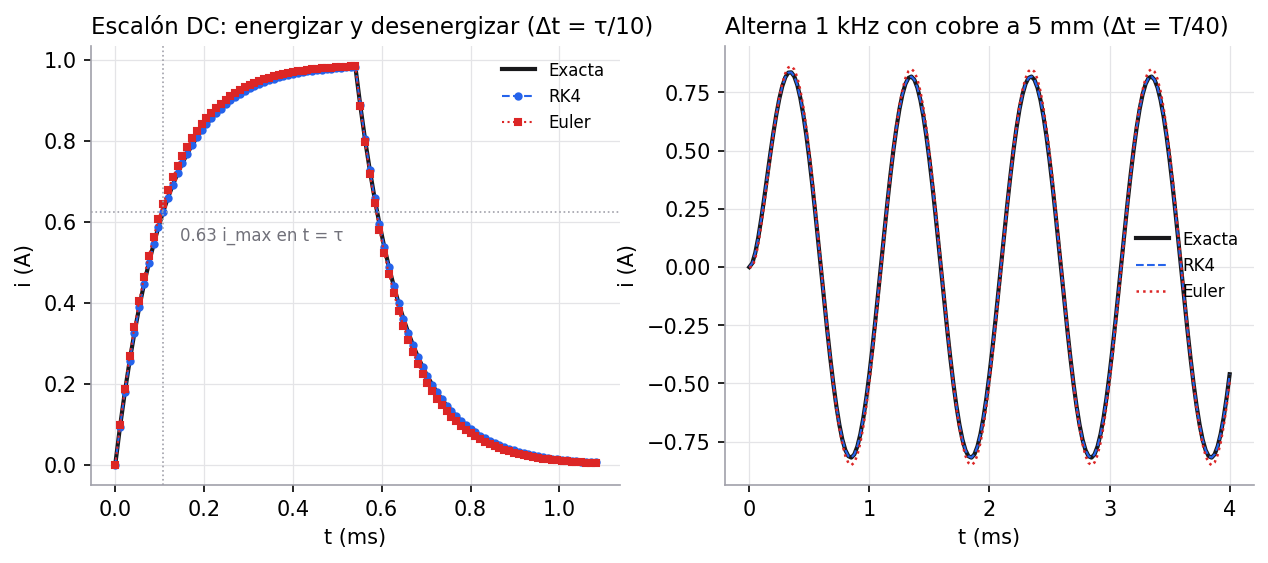
\includegraphics[width=\columnwidth]{respuesta-temporal.png}
    \caption{Corriente con cobre a 5~mm. Izquierda: energizar y desenergizar ($\Delta t=\tau/10$). Derecha:
    alimentación alterna a 1~kHz ($\Delta t=T/40$).}
    \label{fig:simulacion}
\end{figure}

La Figura \ref{fig:campo} muestra el campo de la bobina. Con el cobre, las líneas de $\vec B$ se vuelven paralelas
a la superficie: la componente normal se anula, como exige la condición de frontera de un buen conductor.

\begin{figure}[H]
    \centering
    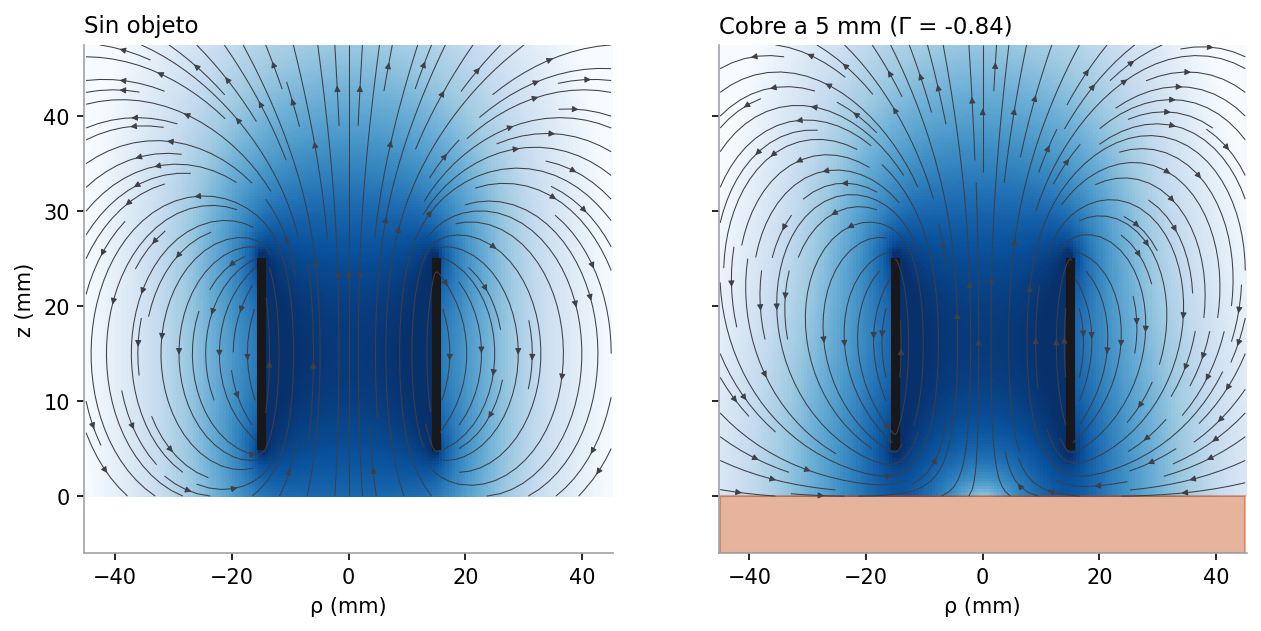
\includegraphics[width=\columnwidth]{campo-magnetico.png}
    \caption{Líneas de campo e intensidad de $\vec B$ sin pieza y con cobre a 5~mm.}
    \label{fig:campo}
\end{figure}

\subsection{Análisis de parámetros}

La sensibilidad de la amplitud a los parámetros se estudia mediante
\begin{equation}
\begin{aligned}
    S_{L}&=\frac{\partial I_p}{\partial L}=-\frac{V_0\,\omega^2L}{(R^2+\omega^2L^2)^{3/2}},\\
    S_{R}&=\frac{\partial I_p}{\partial R}=-\frac{V_0\,R}{(R^2+\omega^2L^2)^{3/2}}.
\end{aligned}
    \label{eq:sensibilidad}
\end{equation}
Con cobre a 5~mm, $S_L=-473.6$~A/H y $S_R=-0.111$~A/$\Omega$: un cambio del 1\,\% en $L$ mueve $I_p$ un 0.32\,\% y
uno del 1\,\% en $R$ un 0.68\,\%. Como el cobre baja $L$ (sube $I_p$) y sube $R$ (baja $I_p$), los dos efectos
compiten. La razón $Q=\omega L/R$ controla qué tanto del cambio de $L$ llega a la corriente: con $N=50$
($Q=0.08$) la señal es de 0.06\,\%, con $N=150$ ($Q=0.75$) de 2.35\,\% y con $N=300$ ($Q=3.0$) de 7.7\,\%.

\begin{figure*}[t]
    \centering
    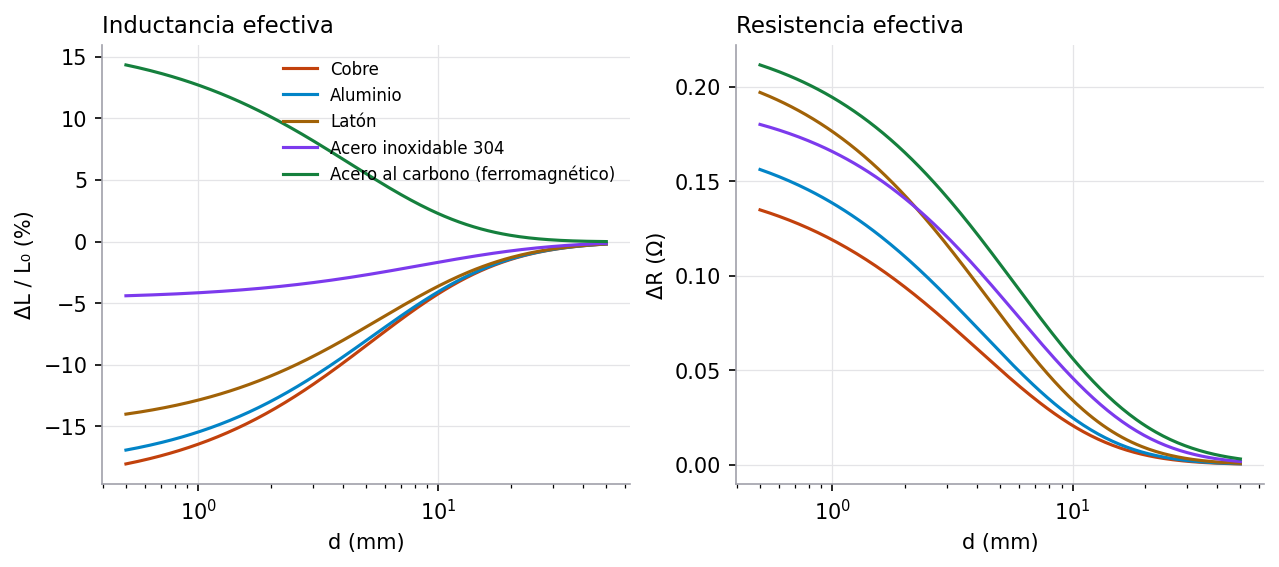
\includegraphics[width=0.49\textwidth]{parametros-vs-distancia.png}\hfill
    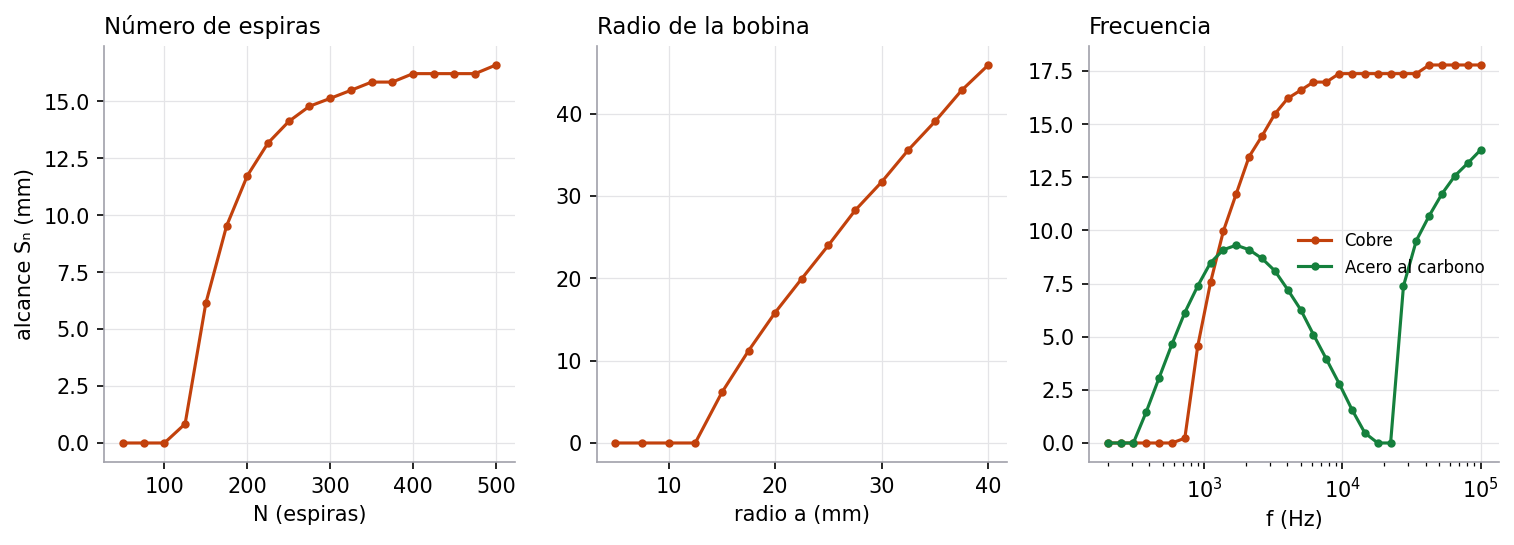
\includegraphics[width=0.49\textwidth]{escenarios-alcance.png}
    \caption{Izquierda: cambio de inductancia y de resistencia frente a la distancia para los cinco materiales.
    Derecha: alcance de detección frente al número de espiras, el radio y la frecuencia.}
    \label{fig:parametros}
\end{figure*}

La Figura \ref{fig:parametros} resume el estudio de escenarios. El alcance crece con el radio de la bobina
($S_n/a\approx1$ para bobinas grandes) porque lejos de ella el campo es el de un dipolo magnético y cae como
$1/z^3$. En frecuencia, el cobre mejora hasta saturarse, mientras que el acero pasa de aumentar la inductancia
(+8.4\,\% a 100~Hz) a disminuirla (−4.0\,\% a 50~kHz): cerca de 20~kHz la magnetización y el apantallamiento se
cancelan y el acero no se detecta (frecuencia ciega).

\usoia{Claude (Anthropic) se usó para programar la interfaz del simulador y los barridos de parámetros. El equipo
definió los escenarios, revisó que los resultados fueran coherentes con la física y los interpretó.}

\section{Resultados y discusión}

\subsection{Presentación de resultados}

La Figura \ref{fig:resultados} presenta la identificación del material. Cada material traza una curva distinta en
el plano de impedancia al variar la distancia; los no ferrosos quedan con fase negativa y el acero con fase
positiva. La matriz de confusión corresponde a 40 piezas por material entre 1 y 8~mm, con ruido de medida de
0.2\,\% en amplitud y 0.1$^\circ$ en fase, dos frecuencias y 16 promedios.

\begin{figure*}[t]
    \centering
    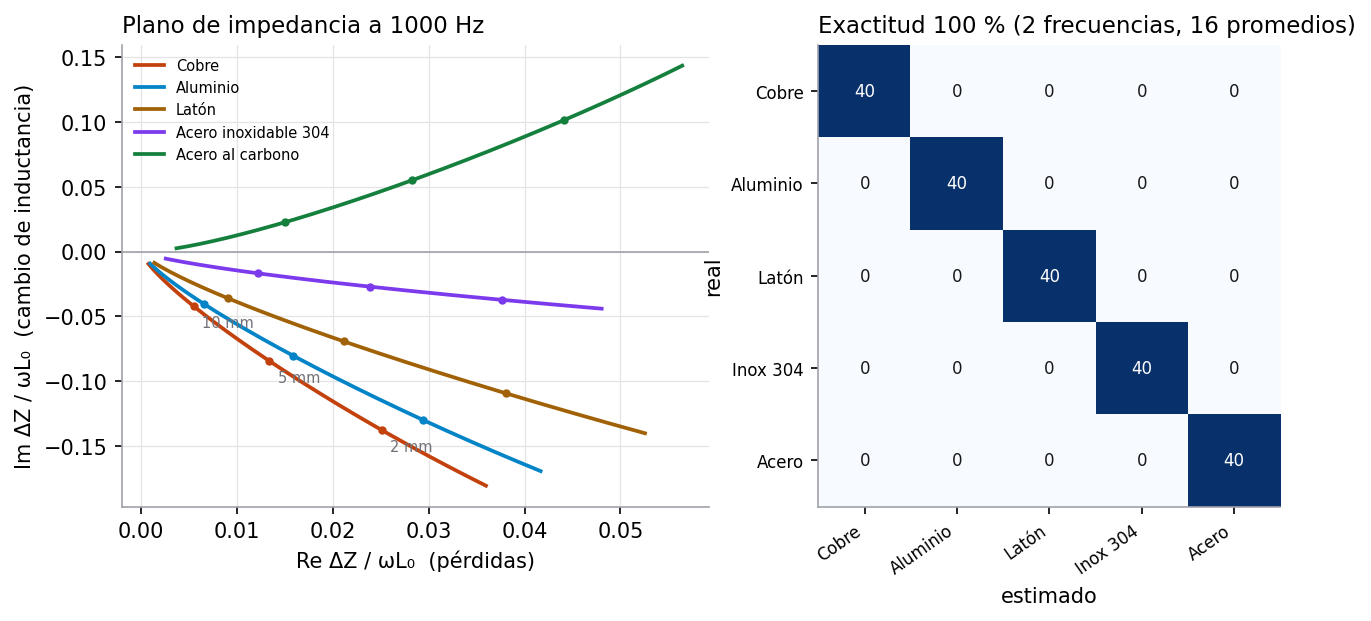
\includegraphics[width=0.82\textwidth]{identificacion.png}
    \caption{Izquierda: plano de impedancia normalizado a 1~kHz (los puntos marcan 2, 5 y 10~mm). Derecha: matriz
    de confusión de la identificación.}
    \label{fig:resultados}
\end{figure*}

\begin{table}[H]
    \centering
    \caption{Respuesta de cada material con la pieza a 5~mm y 1~kHz.}
    \label{tab:materiales}
    \small
    \begin{tabular}{lcccc}
        \toprule
        Material & $\Delta L/L_0$ & $\Delta R$ ($\Omega$) & Fase $\Delta Z$ & $S_n$ (mm) \\
        \midrule
        Cobre & $-8.45$\,\% & 0.050 & $-81.0^\circ$ & 6.1 \\
        Aluminio & $-8.05$\,\% & 0.060 & $-78.8^\circ$ & 5.2 \\
        Latón & $-6.94$\,\% & 0.080 & $-73.0^\circ$ & 1.5 \\
        Inoxidable & $-2.71$\,\% & 0.090 & $-48.5^\circ$ & -- \\
        Acero & $+5.51$\,\% & 0.106 & $+62.8^\circ$ & 7.9 \\
        \bottomrule
    \end{tabular}
\end{table}

\begin{table}[H]
    \centering
    \caption{Exactitud de la identificación (piezas entre 1 y 8~mm).}
    \label{tab:identificacion}
    \small
    \begin{tabular}{lccc}
        \toprule
        Configuración & Material & Ferroso & Error $d$ \\
        \midrule
        1 frecuencia & 84\,\% & 100\,\% & 0.29 mm \\
        2 frecuencias & 89\,\% & 100\,\% & 0.13 mm \\
        1 frec., 16 promedios & 100\,\% & 100\,\% & 0.07 mm \\
        2 frec., 16 promedios & 100\,\% & 100\,\% & 0.03 mm \\
        \bottomrule
    \end{tabular}
\end{table}

\subsection{Comparación de resultados}

La Tabla \ref{tab:comparacion} compara las soluciones analíticas con las numéricas.

\begin{table}[H]
    \centering
    \caption{Comparación de resultados teóricos y numéricos (cobre a 5~mm).}
    \label{tab:comparacion}
    \small
    \begin{tabular}{lccc}
        \toprule
        Magnitud & Teórico & RK4 & Euler \\
        \midrule
        $i(\tau)$, escalón (A) & 0.62582 & 0.62582 & 0.64483 \\
        $I_p$ muestreado, alterna (A) & 0.81848 & 0.81847 & 0.85073 \\
        $q(\tau)$, RC de clase (mC) & 1.13782 & 1.13782 & 1.17238 \\
        Balance de energía (mJ) & 2.1449 & 2.1449 & -- \\
        \bottomrule
    \end{tabular}
\end{table}

En la fila de la alterna se compara el máximo de la solución exacta sobre los mismos instantes de la malla, porque
el máximo muestreado es algo menor que la amplitud teórica $I_p=0.81888$~A de \eqref{eq:amplitud}. La última fila
es la energía entregada por la fuente al energizar, que debe igualar el calor en la resistencia (1.8809~mJ) más la
energía magnética (0.2641~mJ).

\subsection{Discusión de resultados}

\textbf{Correspondencia entre teoría y simulación.} Los casos límite se cumplen: sin pieza $L=L_0$; con un
conductor perfecto $\Gamma\to-1$; con un ferromagnético a baja frecuencia $L$ aumenta; y el efecto desaparece al
alejar la pieza. RK4 reproduce la solución exacta con cinco cifras y conserva la energía con un error de
$5\times10^{-7}$, mientras que Euler, con el mismo paso, se aparta un 3--4\,\%. Las discrepancias se deben al
error de truncamiento de cada método.

\textbf{Evaluación del modelo.} Los fabricantes publican factores de corrección del alcance respecto al acero:
inoxidable $\approx0.7$, latón $\approx0.5$, aluminio $\approx0.4$ y cobre $\approx0.3$ \cite{fericean2007}. Con la
amplitud de la corriente como señal, el modelo acierta en que el acero se detecta más lejos, pero ordena distinto
los no ferrosos, porque la caída de $L$ y la subida de $R$ se compensan parcialmente. Si se ordenan por pérdidas
($\Delta R$, Tabla \ref{tab:materiales}), el modelo da inoxidable $>$ latón $>$ aluminio $>$ cobre, el mismo orden
de los fabricantes. Esto valida el modelo de forma indirecta y explica por qué los sensores comerciales miden las
pérdidas con un oscilador LC.

\textbf{Impacto.} Un solo sensor separa ferrosos de no ferrosos en todas las configuraciones e identifica los
cinco materiales cuando el ruido es bajo. El tiempo de respuesta estimado ($5\tau+3T=3.5$~ms) permite unas
8\,500 piezas por minuto; con 16 promedios y dos frecuencias la medición tarda unos 96~ms, que es el compromiso
entre precisión y velocidad de la banda. De toda la potencia (1.69~W), solo el 1\,\% se disipa en la pieza, y es
esa fracción la que produce la señal.

\textbf{Limitaciones.} La pieza se supone infinita; una pieza delgada o pequeña acopla menos, y resolverlo exige
elementos finitos. La bobina no tiene núcleo de ferrita. Los materiales son lineales. Además, el sensor solo ve
$\sigma$ y $\mu_r$: un cobre con el 60\,\% de su conductividad es indistinguible del aluminio, y una impureza que
reduzca la conductividad un 20\,\% desplaza la firma apenas un 1.5\,\%, detectable solo con ruido muy bajo.

\subsection{Análisis del error}

La diferencia porcentual entre los resultados teóricos y numéricos se calcula como
\begin{equation}
    \varepsilon(\%)=
    \frac{|R_{\mathrm{teórico}}-R_{\mathrm{numérico}}|}
    {|R_{\mathrm{teórico}}|}
    \times 100 .
    \label{eq:error_porcentual}
\end{equation}
Para $i(\tau)$ en la Tabla \ref{tab:comparacion}, RK4 da $\varepsilon<10^{-4}$\,\% y Euler $\varepsilon=3.0$\,\%;
para la amplitud alterna, RK4 da $0.001$\,\% y Euler $3.9$\,\%. En el balance de energía, la diferencia de RK4 es
$5\times10^{-5}$\,\%.

\usoia{Claude (Anthropic) se usó para generar las tablas y figuras a partir del código y para redactar un borrador de
la discusión. La interpretación física, la comparación con los sensores comerciales y la identificación de las
limitaciones fueron revisadas y validadas por el equipo.}

\section{Conclusiones}

\begin{enumerate}
 \item El sensor se modeló desde las leyes de Faraday y Ampère, usando solo las ecuaciones de Maxwell necesarias,
       y su circuito RL se resolvió con el mismo procedimiento del circuito RC de clase. Se cumplieron los objetivos
       de deducción y solución analítica.
 \item Euler y RK4, programados manualmente, convergen con órdenes 1.01 y 4.02, conservan la energía (RK4 con error
       de $5\times10^{-7}$) y reproducen el ejercicio RC de clase. RK4 alcanza un 1\,\% de error con dieciséis veces
       menos pasos que Euler.
 \item La pieza conductora reduce la inductancia y la ferromagnética la aumenta a baja frecuencia. El alcance es del
       orden del radio de la bobina y el acero tiene una frecuencia ciega cerca de 20~kHz.
 \item La fase del cambio de impedancia identifica el material y su magnitud da la distancia: con dos frecuencias y
       16 promedios se identifica el 100\,\% de las piezas con un error de distancia de 0.03~mm. Separar ferrosos de
       no ferrosos es robusto en todos los casos.
 \item Como mejoras se proponen medir las pérdidas en lugar de la amplitud, usar una medición diferencial para
       detectar impurezas y extender el modelo a piezas finitas y bobinas con núcleo mediante elementos finitos,
       validándolo con un prototipo.
\end{enumerate}

\usoia{Las conclusiones se redactaron con apoyo de Claude (Anthropic) a partir de los resultados del proyecto y
fueron revisadas por el equipo.}

\section{Referencias}

% La sección ya tiene título: se omite el encabezado propio de la bibliografía
\begingroup
\renewcommand{\section}[2]{}
\begin{thebibliography}{99}

\bibitem{dodd1968}
Dodd, C. V., y Deeds, W. E.
``Analytical solutions to eddy-current probe-coil problems.''
\textit{Journal of Applied Physics}, vol. 39, no. 6, pp. 2829--2838, 1968.

\bibitem{wheeler1928}
Wheeler, H. A.
``Simple inductance formulas for radio coils.''
\textit{Proceedings of the IRE}, vol. 16, no. 10, pp. 1398--1400, 1928.

\bibitem{griffiths2017}
Griffiths, D. J.
\textit{Introduction to Electrodynamics}, 4.\textsuperscript{a} ed.
Cambridge University Press, 2017.

\bibitem{jackson1999}
Jackson, J. D.
\textit{Classical Electrodynamics}, 3.\textsuperscript{a} ed.
John Wiley \& Sons, 1999.

\bibitem{serway2018}
Serway, R. A., y Jewett, J. W.
\textit{Física para ciencias e ingeniería}, vol. 2, 10.\textsuperscript{a} ed.
Cengage Learning, 2018.

\bibitem{libby1971}
Libby, H. L.
\textit{Introduction to Electromagnetic Nondestructive Test Methods}.
Wiley-Interscience, 1971.

\bibitem{garcia2011}
García-Martín, J., Gómez-Gil, J., y Vázquez-Sánchez, E.
``Non-destructive techniques based on eddy current testing.''
\textit{Sensors}, vol. 11, no. 3, pp. 2525--2565, 2011.

\bibitem{fericean2007}
Fericean, S., y Droxler, R.
``New noncontacting inductive analog proximity and inductive linear displacement sensors for industrial
automation.''
\textit{IEEE Sensors Journal}, vol. 7, no. 11, pp. 1538--1545, 2007.

\bibitem{burden2017}
Burden, R. L., Faires, J. D., y Burden, A. M.
\textit{Análisis numérico}, 10.\textsuperscript{a} ed.
Cengage Learning, 2017.

\bibitem{butcher2016}
Butcher, J. C.
\textit{Numerical Methods for Ordinary Differential Equations}, 3.\textsuperscript{a} ed.
John Wiley \& Sons, 2016.

\bibitem{virtanen2020}
Virtanen, P., et al.
``SciPy 1.0: fundamental algorithms for scientific computing in Python.''
\textit{Nature Methods}, vol. 17, pp. 261--272, 2020.

\bibitem{harris2020}
Harris, C. R., et al.
``Array programming with NumPy.''
\textit{Nature}, vol. 585, pp. 357--362, 2020.

\bibitem{meurer2017}
Meurer, A., et al.
``SymPy: symbolic computing in Python.''
\textit{PeerJ Computer Science}, vol. 3, e103, 2017.

\bibitem{hunter2007}
Hunter, J. D.
``Matplotlib: a 2D graphics environment.''
\textit{Computing in Science \& Engineering}, vol. 9, no. 3, pp. 90--95, 2007.

\bibitem{icesi_guia}
Universidad Icesi.
\textit{Guía de proyectos de Electromagnetismo} y apuntes de clase (circuito RC, ley de Gauss, campos eléctricos en
la materia, pantallas táctiles capacitivas). Cali, 2026.

\bibitem{anthropic2026}
Anthropic.
\textit{Claude} (modelo de lenguaje), usado mediante Claude Code. 2026. Disponible en:
\url{https://claude.ai}.

\end{thebibliography}
\endgroup

% =================================================
% OBSERVACIÓN SOBRE EL USO DE INTELIGENCIA ARTIFICIAL
% =================================================

\vspace{0.3cm}
\noindent
\textbf{OBSERVACIÓN SOBRE EL USO DE INTELIGENCIA
ARTIFICIAL (IA)}

\vspace{0.1cm}

\noindent
En el desarrollo del proyecto se usó Claude (Anthropic) \cite{anthropic2026}, mediante Claude Code, como
asistente de programación y de redacción. Su uso se declara al final de cada apartado. La herramienta apoyó la
escritura del código (modelo físico, métodos numéricos, identificación y simulador), la generación de figuras y
tablas, y los borradores de las deducciones y del texto. Los autores definieron el problema y el caso de estudio,
contrastaron las deducciones con los apuntes de clase, ejecutaron y verificaron los cálculos (solución exacta,
SciPy, pruebas automáticas y balance de energía) y son responsables de la veracidad, validez, interpretación y
calidad de los contenidos presentados.

\vspace{0.3cm}
\noindent
\textbf{OBSERVACIÓN SOBRE LOS DESARROLLOS NUMÉRICOS
Y COMPUTACIONALES}

\vspace{0.1cm}

\noindent
El código fuente, las pruebas, el script que genera las figuras y el simulador están en el repositorio
\url{https://github.com/luisrodriguez-rgb/Proyecto-Final-Fisica}. Para reproducirlos:
\texttt{python3 -m venv .venv}, \texttt{.venv/bin/pip install -r requirements.txt} y
\texttt{.venv/bin/streamlit run app.py}. Las pruebas se ejecutan con \texttt{pytest} y las figuras con
\texttt{scripts/generar\_figuras.py}. El informe extendido por criterio de la rúbrica está en la carpeta
\texttt{docs/}.

\end{document}
